%%%%%%%%%%%%%%%%%%%%%%%%%%%%%%%%%%%%%%%%%
% University/School Laboratory Report
% LaTeX Template
% Version 3.1 (25/3/14)
%
% This template has been downloaded from:
% http://www.LaTeXTemplates.com
%
% Original author:
% Linux and Unix Users Group at Virginia Tech Wiki 
% (https://vtluug.org/wiki/Example_LaTeX_chem_lab_report)
%
% License:
% CC BY-NC-SA 3.0 (http://creativecommons.org/licenses/by-nc-sa/3.0/)
%
%%%%%%%%%%%%%%%%%%%%%%%%%%%%%%%%%%%%%%%%%

%----------------------------------------------------------------------------------------
%	PACKAGES AND DOCUMENT CONFIGURATIONS
%----------------------------------------------------------------------------------------

\documentclass{article}

\usepackage[version=3]{mhchem} % Package for chemical equation typesetting
\usepackage{siunitx} % Provides the \SI{}{} and \si{} command for typesetting SI units
\usepackage{graphicx} % Required for the inclusion of images
\usepackage{natbib} % Required to change bibliography style to APA
\usepackage{amsmath} % Required for some math elements 
\usepackage{todonotes}
\usepackage{wrapfig}
\usepackage{caption}
%\usepackage{chemmacros}
\usepackage[export]{adjustbox}
\usepackage{pbox}
\usepackage{eurosym}
\usepackage{listings}
\lstset{
captionpos=b,
language=c,
stepnumber=2,
tabsize=2,
frame=single,
label=DescriptiveLabel,
% upquote=true,
aboveskip={1.5\baselineskip},
columns=fullflexible,
showstringspaces=false,
extendedchars=true,
breaklines=true,
showtabs=false,
showspaces=false,
showstringspaces=false,
% identifierstyle=\ttfamily,
% keywordstyle=\footnotesize,
% keywordstyle=\font\ttfamily,
% keywordstyle=\color[rgb]{0,0,1},
% commentstyle=\color[rgb]{0.133,0.545,0.133},
% stringstyle=\color[rgb]{0.627,0.126,0.941},
% basicstyle=\color[rgb]{0,0,0},
basicstyle=\footnotesize,
}
\usepackage{geometry}
\newgeometry{left=2cm, right=2cm, bottom=2cm, top=3cm}
\setlength\parindent{0pt} % Removes all indentation from paragraphs

\renewcommand{\labelenumi}{\alph{enumi}.} % Make numbering in the enumerate environment by letter rather than number (e.g. section 6)

%\usepackage{times} % Uncomment to use the Times New Roman font

%----------------------------------------------------------------------------------------
%	DOCUMENT INFORMATION
%----------------------------------------------------------------------------------------

% \title{Energy Aware Software} % Title

% \author{\textbf{Principal investigator}: Simon Holmbacka\\ \AA{}bo Akademi University, Embedded Systems Laboratory} % Author name


\begin{document}
\huge{Energy Aware Software}
% \normalsize\textbf{Principal investigator}: Dr. Simon Holmbacka\\ 
% \textbf{Project starting time}: 01.09.2017\\
% \textbf{Duration of the project}: 48 months\\
% \textbf{Site of research}:\\
% \textit{\AA{}bo Akademi University} \\
% \textit{Faculty of Science and Engineering}\\
% \textit{Embedded Systems Laboratory}\\
% \textit{Vattenborgsv\"{a}gen 5 20500 Turku, Finland}\\

\begin{table}[h]
\begin{tabular}{  l  l  }
\pbox{15cm}{\normalsize\textbf{Principal investigator}: Dr. Simon Holmbacka\\\textbf{Project starting time}: 01.09.2018\\\textbf{Duration of the project}: 48 months\\} & 
\pbox{10cm}{\textbf{Site of research}:\\\textit{\AA{}bo Akademi University (AAU), Turku, Finland}\\\textit{Faculty of Science and Engineering}\\\textit{Embedded Systems Laboratory}}
 
\end{tabular}
\label{tab:strconf}
\end{table}
\normalsize
\textbf{Sites for research cooperation:}
\begin{table}[h]
\begin{center}
\begin{tabular}{  l  l  }
\pbox{10cm}{\textit {IETR - INSA Rennes }
\includegraphics[width=0.4cm]{fig/fra.png} \\\textit {Institut d'Electroniques et de T\'{e}l\'{e}communications}\\\textit{Rennes,  France}} & 
\pbox{10cm}{\textit {TU Wien }
\includegraphics[width=0.4cm]{fig/aus.png} \\ \textit{Institute for Software Technology and Interactive Systems}\\\textit{Vienna, Austria}}   \\ \\
\pbox{10cm}{\textit{FernUniversit\"{a}t in Hagen }
\includegraphics[width=0.4cm]{fig/ger.png} \\ \textit{Fakult\"{a}t f\"{u}r Mathematik und Informatik}\\ \textit{Hagen, Germany}} & 
\pbox{10cm}{\textit{Uppsala University }
\includegraphics[width=0.4cm]{fig/swe.png} \\\textit{Department of Information Technology}\\\textit{Uppsala, Sweden}} \\ 
\end{tabular}
\label{tab:strconf}
\end{center}
\end{table}

\date{\today} % Date for the report

% \maketitle % Insert the title, author and date
\normalsize
\vspace{-0.9cm}
\section{Rationale}
Energy consumption is currently a challenge in all domains of computer systems.
% IoT, cyber physical systems and other mobile systems demand solutions to lower the energy consumption while keeping the same amount of computations,
% and high end systems, servers and exa-scale computing demand more computations for the same energy.
From tiny embedded systems to large scale server farms and diverse IoT systems, energy efficiency is becoming the main struggle for system usability, expansion, reliability and scalability.
The drivers for solving the issues differ depending on the area of focus;
the very usability of battery powered devices depends on its ability to provide the user with the satisfactory experience while consuming the minimal amount of energy.
Desktop and laptop systems require high levels of energy efficiency in order to (a) lower noise levels from active cooling, (b) increase the reliability by reducing the heat and (c) minimize the electric bill.
Taking into account the bigger picture, the rapid expansion of large scale servers is not in line with ecological development, and now contributes to over 2\% of the total energy consumption in the US\footnote{Statistics according to the U.S. Office of Energy Efficiency \& Renewable Energy: http://energy.gov/eere/femp/resources-data-center-energy-efficiency}, with Facebook alone releasing 650k tonnes of carbon annually\footnote{https://sustainability.fb.com/en/our-footprint/}.
Lastly, without increased energy efficiency, high performance computing centers cannot reach exa-scale performance.
The US Department of Energy\footnote{http://ascr-discovery.science.doe.gov/2014/11/exascale-road-bumps/} have defined a maximum power envelope of 20 MW for a single data center, but with current technology, a modern exa-scale computing center would require over 7000 MW.\smallskip

These problems were traditionally solved by the hardware evolution.
The clock frequency wall was avoid in the beginning of the 2000s by the introduction of multi-core based systems. 
This led to a new challenge in mid-2000s: the CPU power wall \cite{Danowitz:12,Wang:13}. 
Indeed, due to physical limitations of semiconductor materials, the power dissipation of a fixed chip area is limited. 
With the evolution in the fabrication of semiconductor devices, from a 10$\mu$m manufacturing process in the 70s until the commercialization of 10nm based technology in 2017 (in e.g. the Samsung Galaxy S8), more transistors are squeezed into a smaller silicon area which increases power density \cite{5514312}. 
This eventually leads to dark silicon, when all the components of a chip can not be operated at the same time due to both its power dissipation and generated heat. 
The effects of the power wall was until now limited by the design of more energy efficient transistors with for example lower voltage levels,
which has led to an increase in the transistor efficiency in proportion to an increase of transistor density -- a phenomenon called the Dennard scaling \cite{Dennard:74}. 
However the current increase of the transistor efficiency is not any more proportional to the increase of transistor density \cite{Wang:13}, 
and the semiconductor device fabrication is currently in a post-Dennard scaling area, where a substantial increase of the performance of computing
systems cannot be achieved until both the current power dissipation and the related energy consumption issues are resolved.\smallskip

In eradicate the above-mentioned constraints in this interdisciplinary domain, specific software must inevitably be introduced to make computer systems energy efficient again!
The vision behind this research is to significantly improve the energy efficiency of computer systems by involving the application software in the decision of allocating resources -- this branch of self-awareness is called ``\textbf{making the software energy-aware}''.
Energy-aware software form a stronger link between applications and the runtime system by means of an information flow used to steer the allocation of resources,
which increases the self-awareness of software. This advancement in software design is required for the research community to take the next step into energy efficient computing.\smallskip

The key challenge is to utilize the available hardware resources as efficiently as possible.
Since general purpose applications behave in a very dynamic way, a runtime environment must continuously adjust the usage of the resources based on the execution of the applications.
In Linux based systems, attempts have been made to incorporate this behavior by using clock frequency scaling and deep sleep states to scale the hardware resources according to the demand. 
The limitations with the existing approaches are that the resources are allocated based on poor metrics.
There is no interoperability between applications and the runtime system, and resources are usually allocated based on indirect metrics such as the system \textit{workload}.
Such a metric does not describe performance demands in applications, and therefore often causes incorrect resource allocation,
which, in turn, leads to and additional waste of energy \cite{HolmbackaDasip, HolmbackaHipeac}.
In other words, the software is currently not energy-aware.
\smallskip

\begin{wrapfigure}{br}{8.5cm}
%   \begin{center}
%     \vspace{-0.8cm}
    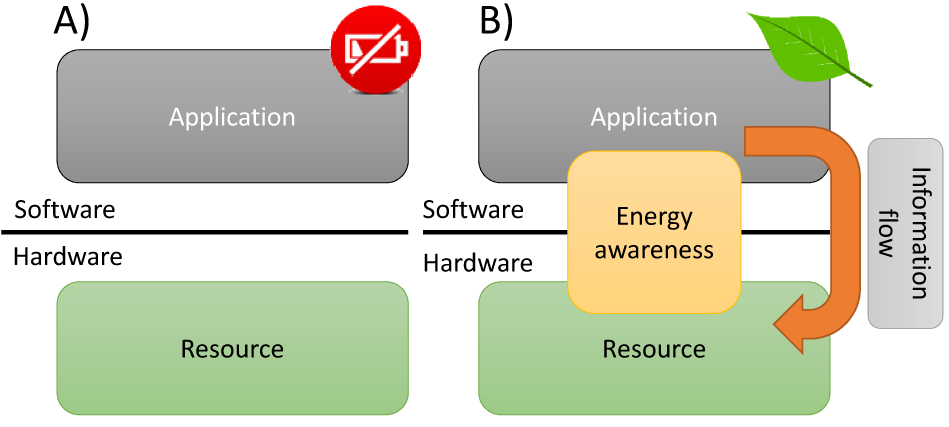
\includegraphics[width=8.0cm]{fig/EAS_Overview.png}
%   \end{center}
  \caption{A: No connection between the application and the resources B: Resource allocation based on self-awareness}
  \label{fig:EAS}
%   \vspace{-2cm}
\end{wrapfigure}

%\todo[inline,color=green]{Here comes what we do in this research:}
In this research project we will enhance the application software with the inclusion of \textit{energy-awareness}.
This new property will enable applications to get directly involved in the allocation of resources.
Energy-aware software is able to continuously report the performance demand in its own specific metric to the runtime system.
With this new vital information, the runtime system is able to allocate resources (usually with clock frequency scaling and with sleep states) with a much greater accuracy than using indirect metrics such as the workload.
As a result of the inclusion of energy-awareness in software on real-world Linux platforms in our previous research \cite{Holmbacka:15}, an impressive saving of 50\%-60\% in energy was achieved -- 
without compromising on the performance!
We are therefore confident that adding energy-awareness in general purpose software can reduce the energy consumption significantly.
Figure~\ref{fig:EAS} illustrates the purpose of the research: part A) shows the current approach without any interoperability between applications and the resources, i.e. no energy-awareness.
Using this approach, resources are allocated based on the level of workload or other indirect means of metric.
Part B) in Figure~\ref{fig:EAS} illustrates the inclusion of energy-awareness. 
This is the added interface between the application and the runtime system through which the application communicates.
It results in a better accuracy of resource allocation by increased in self-awareness and leads to lower energy consumption.\smallskip

The research area in energy efficient computing is a broad domain spanning several levels of hardware from IoT to Exascale.
The commonality is, however, the ability to propagate information from the highest software layer to the runtime system, and to the hardware.
Throughout all computing domains in the area of energy efficient computing, we have identified three critical challenges to address in our research further specified in the following paragraphs.

\paragraph{Challenge 1: Self-awareness}
\label{sec:self}
Applications must be able to properly express their intentions in terms of performance requirements during execution. 
% Such requirements are added to the application software in form of performance meta-data -- a performance goal the application is due to achieve. 
The challenge is therefore to provide a framework with the capability of handling and expressing proper performance data in an interdisciplinary domain.
% As previously mentioned, the traditional way of solely monitoring the workload is a very inaccurate and often counter-productive both in terms of performance and energy.
% We tackle this challenge by allowing the applications to express the resource requirements internally.
This means that the application should include a small part of code -- the meta-data -- which expresses the intention of the application in its own understanding of performance.
For example, the end user of a video decoder is satisfied in case the decoder produces a framerate of 25 fps because of properties in the human eye and the understanding of moving pictures. 
A higher framerate is therefore energy waste while not producing any higher satisfaction for the end user.
% Therefore, we will investigate the types on meta-data needed to describe the intentions of an application sufficiently accurate.
These type of meta-data must have a sufficiently descriptive form, which can be generalized to any new- or legacy application.
% Once the meta-data descriptions have been established, the injection of the data into both new- and legacy applications must be achieved fairly effortless in order for the programmers to make the additional effort.
% A trade-off between descriptiveness and programmer effort is to be expected, since the intension

\paragraph{Challenge 2: Interoperability}
\label{sec:inter}
The interoperability challenge in the domain of energy-awareness in application software is to create an ecosystem capable of exchanging information about the intentions of an application to the resource allocation layer. 
% The exchanged information must be interpreted by the runtime layer to make sensible decisions regarding the resource allocation.
Since applications in general are dynamic, the performance of the application depends on a wide set of factors such as memory intensity, use of caches, user interrupts, the data sizes and data types used, interaction with other applications etc. 
This means that the performance of an application cannot be guaranteed with fixed resources, and online interoperability must guarantee proper information between the running application and the resource allocation.
To ensure this, the application must be monitored at runtime, and steps must be taken in case the resource demand is not in line with the resource allocation.
% In case the currently allocated performance is either too high or too low, the monitor reports this issue to the controller which allocates or deallocates resources to accommodate for the real resource requirement.
% We recognize therefore the need for a proper monitoring framework to insure the interoperability between applications and the runtime system.
Such a framework must be detailed enough and provide sufficient tools for measuring performance, but simple enough to reduce programmer effort for using it.
Since the monitoring framework is a runtime system, a considerably low overhead must be guaranteed to avoid interference with the energy consumption and performance of the host system.

\paragraph{Challenge 3: Smart adaptivity}
\label{sec:smart}
Given a proper dataflow from applications to the runtime system, the final challenge is the allocation of resources. 
Allocating resources efficiently means having knowledge of how the resources of one form affects the performance of the application requesting the resources.
The methods must be adapted and applied to the general purpose computing domain. 
A considerable challenge is to design a scalable control system, which is generic enough to fit into different sizes of computer systems, yet specific enough to handle platform specific actuators and capabilities, whether it is PID controllers, fuzzy controllers or machine learning-based controllers.

\subsection{Previous work}
The PI has for the last seven years focused on low power and energy-aware software. 
It has been noted that the trend of performance requirements by far exceeds e.g the battery capacity of a mobile device, especially since the mobile multi-core revolution \cite{BatteryCapacity,CPUCapacity}. 
% This means that the performance of the hardware and the demand for performance of the user is greater than the energy a battery with limited dimensions can physically store.Fwhich  
Because of the slow capacity increase in batteries, the available energy must be used more efficiently in order for such a mobile device to retain its usability.
In the thesis of the PI ``\textit{Energy Aware Software for Many-Core Systems}'' two guidelines were presented for creating energy-aware software on modern many-core hardware. 
Implementing the recommendations in software has proven to reduce the energy consumption up to 50\% without degrading the performance \cite{HolmbackaHipeac}, especially on mobile multi-core hardware. 
The recommendations called ``Energy-aware mapping'' and ``Energy-aware resource allocation'' are used to tailor the resource allocation to the software executing, 
and a prototype runtime system was implemented as a phase of the PhD thesis.
More specifically, the recommendations allow the system to use the optimal number of cores and the optimal clock frequency according to the performance requirement of the running application.
Using this software, practical state-of-the-art demonstrators were created, for example a low power video transcoding cloud system\footnote{Picture of the ESLab demonstrator available at https://dl.dropboxusercontent.com/u/5260559/ClusterDemo.jpg} demonstrated in the Millennium Pavilion SHOK Summit 2014 in Helsinki, and in the DIGILE Workshop 2013 ``Rolling up the Sleeves''.
Also, the Android app ``Low Energy Player'' was implemented as a state-of-the-art demonstrator and is available on Google store\footnote{https://play.google.com/store/apps/details?id=org.videolan.vlc.LEL.lite.green}
This research project reaches beyond the state-of-the-art by the development of a programming framework for energy-aware software ready to use by the everyday-programmer, 
which has not been available to this date.
Therefore, the proposed research project has a perfect fit with the PI's previous involvement in research and the ability for a breakthrough in the field is expected.
\subsection{Related work}
The concept of ``low energy programming'' or ``low power programming'' has previously existed in the form focusing on the programming paradigm or on the programming syntax. 
Guidelines from Intel \cite{IntelLowPower} suggests the use of a certain level of loop unrolling, vectorization, memory intensity cache usage etc.
for achieving maximum energy efficiency in combination with Intel compiler tools. 
Such recommendations are applied only on the algorithms in the program, and do not cover, the intention of the program for functioning efficiently together with the runtime system allocating the resources. 
The low power programming guidelines from Intel also require the programming to construct the program in a certain way in order to become energy efficient, 
and the underlying hardware architecture must be known. 
In the thesis ``Developing Energy-Aware Software'' by Brinke \cite{Brinke:15} the author describes programming languages for modularity and modeling resource consumption for software.
The \textit{awareness} of energy, is tightly bound to the application code and the programmer is expected to follow certain programming patterns to make the software energy-aware.
On the contrary, the planned framework for energy efficient software requires only the insertion of meta-data in the software.
This means minimal effort of the programmer and the application algorithms can be implemented without interference from the energy-awareness framework.
The resource requirements are specified using a simple library, where after the runtime environment allocates the required resources.\smallskip

\paragraph{Related projects.}
Our newly funded AKA project \textbf{Efficient Stream Computing (2017-2021 799k \euro)} introduces a formal and practical paradigm of measuring efficiency of software execution through the notion of \textit{Fitness},
which characterizes how much of the microarchitecture the task is able to exploit.
This will enable the optimization of Stream Computing systems for energy efficiency, performance or cost with minimal overhead in the development.
The commonality of this project is energy efficient execution, but while ESC focuses more on \textit{where to map} a task, the primary goal of this project is to optimize resource allocation and how software can influence this decision. \smallskip

The \textbf{Carbon Research Group}\begin{small}{ (http://groups.csail.mit.edu/carbon/)} \end{small} at MIT has developed a heartbeat framework to evaluate performance as a generic parameter in software construction.
The framework is capable of measuring performance of any application as a generic parameter by user inserted API calls to the heartbeat library. 
Measuring performance is the necessary first step when constructing a feedback-based control system. 
For example it enables the possibility to measure the framerate in a video decoder, but a controller is then needed to allocate the resources in order to keep the performance on a given setpoint. 
We consider using the heartbeat framework for measuring generic performance in our energy-awareness framework, 
but we plan to extend the framework considerably in order to add the controller for allocating resources.\smallskip

The \textbf{Hardkernel} project\begin{small}{ (http://www.hardkernel.com/main/main.php)} \end{small} creating the Odroid family boards recently released the Global Task Scheduling (GTS) support for the ARM big.LITTLE devices. ``High performance threads'' are scheduled to the big high performance cores and ``Low performance threads'' are scheduled to LITTLE energy efficient cores based on the workload activity of the threads in order to save energy. 
Even though the activity level of a thread is an early attempt introduce energy-awareness in the system, the practical results are poor. 
In other words, the scheduler most often schedule a thread on \textit{the wrong core}. 
This results not only in energy inefficiency, but also in poor performance of the applications and an unsatisfactory user experience.
We will use this platform as one of the reference models for our energy-awareness framework because its SoC is very popular and is being used in millions of Android devices worldwide.\smallskip

Our research group is currently a partner in the \textbf{INTERSYS (2016-2017 496k) \euro} project\\ \begin{small}{ (http://iot4health.utu.fi/?p=374)} \end{small} dedicated to standardize and optimize interconnected IoT devices handling streaming data. Since the number of IoT devices are expected to rapidly increase in the near future, the project is extending interoperability notions for handling the massive amount of data streams from small devices to gateways and servers. 
Still missing is the notion of energy-awareness, which is a crucial point as most devices operate on battery-only power. 
We intend to work closely with this project and we plan to introduce the benefit of energy-awareness into IoT systems.\smallskip

\textbf{EMBECOSM}\begin{small}{ (http://www.embecosm.com/)} \end{small} focus on providing the GCC compiler with the notion of energy efficiency, in practice this means learning which compiler flags minimize the energy consumption for a selected architecture. 
The outcome of this project is similar to OpenTuner \begin{small}{ (http://opentuner.org/)} \end{small} from MIT, which is capable of offline optimization of multi-criteria problems. 
Both projects provide a metric for offline optimization but runtime support, which we suggest, is not stated in their scope. 
Runtime optimization is critical in virtually any environment containing multi-node and heterogeneous multi-node platforms. 
This is because the data used in especially streaming applications like multi-media software is arbitrary or very difficult to predict. 
Compile time optimizations can for example not predict what kind of video format is being used in a video decoder.\smallskip

The \textbf{StarPU}\begin{small}{ (http://starpu.gforge.inria.fr/)} \end{small} project at INRIA Bordeaux and the \textbf{PEPPHER}\begin{small}{ (http://www.peppher.eu/)} \end{small} project has presented a runtime system to minimize the performance for heterogeneous architectures. 
The system builds a performance model of the implemented CUDA or OpenCL kernels based on benchmarking on CPUs and GPUs, after which the system is able to schedule the kernels onto the most performance efficient device. However, they only consider the optimizations in form of performance, not energy efficiency.\smallskip

Therefore, whilst there are a number of ongoing projects researching energy efficiency in general, none of them so far has endeavored to solve the problem of increasing energy efficiency with energy-aware applications.

 
{small}

\paragraph{Related work.}
In previous work, Eyerman et al. \cite{Eyerman:09} claim that no single throughput metric is fundamentally generic for multiprogram workloads. 
Performance should instead be expressed as related to the internal single case-study; a direction adopted in this research. 
However, we plan to integrate this direction of thinking into user defined meta-data that expresses resource requirements in software.\smallskip

A high-level language CQML \cite{Aagedal:01} was suggested for describing QoS requirements integrated in UML. 
CQML links a high level QoS description to system performance, and can describe system actions based on the result. 
Applications specify a performance setpoint and a lower bound acceptable performance level in context of the application. 
Applications then monitor own performance and signal this value to the QoS manager periodically. 
We will consider a similar structure to define QoS in our framework, but more focus will put on the link between applications and hardware resources in a single computer system.
On the contrary, our methods for energy-aware programming will not be strongly tied to a certain programming language and the framework itself will have the flexibility to be integrated from various environments such as servers and PCs and Android.\smallskip

Runtime systems for minimizing energy consumption in computer systems have been previously proposed.
The PowerDial \cite{Hoffmann:11} approach allows graceful degradation in applications based on current application performance measured in heartbeats \cite{Hoffmann:10}. 
The system transforms application parameters (such as peak-signal-to-noise in a video) into dynamic control variables stored in the application itself. 
A callback function is inserted into the application, which the controller uses to adjust the control variables according to performance and policies.
A heartbeat feedback monitors the execution and reports on the updated performance of the application. 
Also, the work by Segovia \cite{Segovia:11} suggests graceful degradation of the application QoS by monitoring a \textit{happiness} value in the application. 
Based on this value, the runtime system can degrade quality points in the application in order to achieve the requested QoS. 
Our planned runtime system is inspired by the same approach to treat input signals from applications: the performance is transformed into a generic parameter – QoS – upon which the controller acts.
In contrast, our controller uses no graceful degradation in the applications, but the actual hardware actuators to allocate resources.\smallskip

There has previously been a strong separation between monitor and control.
Several research projects offer the opportunity to monitor an executing application, but supports no control of the hardware.
On the other hand, many controller-based research project do not support any proper framework for declaring meta-data requirements and monitoring of the execution.
This research project will tie both parts together with the main focus on reducing the energy consumption with minimal programmer effort -- an effort not previously emphasized.
Our research project will also ensure a proper balance between academic research and practical usability,
which means that there is both a focus on planning the long term usage of the framework in terms of capabilities and scalability, but also practical efforts to enable a programmer to pick up the tools and start developing energy-aware software in the industry.
\section{Scientific Objectives and Expected Impact}
\subsection{Scientific objectives}
\paragraph{Objectives of the project and their theoretical and methodological underpinnings.}
Our objective is to solve the energy consumption problem in computer systems, and it is divided into three main scientific objectives:
1) increasing the self-awareness in applications by introducing energy-awareness using a provided programming framework, 
and 2) exposing the features of energy-awareness by interoperability between the user, the application and the runtime system, 3) implementing smart-adaptivity in form of a runtime system capable of optimally allocating the available resources based on the performance demands in the application. \smallskip

In most recent systems, power managers have been implemented to scale the performance of the system according to the current resource demand.
In mainstream Linux systems, the resource demand is measured as the utilization caused by the workload of the CPU. 
Various implementations exist both for large cloud farms or a small IoT systems, 
but main constraint in current solutions is the inability to express resource demands \textbf{explicitly in applications}, hence applications are not currently energy-aware.
In general computer systems, high workload does not necessary mean that an application requires more performance, it simply describes how much the application is using the CPU.
It is merely an indirect effect of executing an application.
Incorrect resource allocation results in either poor performance or in energy waste.\smallskip

% Workload in operating systems is measured as a sliding window average over an active and idle CPU as illustrated in Figure~\ref{fig:workload}. 
% A high workload indicates that the system needs more resources, and the clock frequency is scaled up to decrease the workload of the CPU.
% Setting the frequency can be based on different policies implemented in \textit{frequency governors}, and the most common policy is called ``ondemand''\cite{ondemand}.
% This frequency governor scales the clock frequency to the maximum value as soon as a workload threshold is reached.
% After this it step-wise decreases the clock frequency to the lowest frequency not exceeding the threshold.\smallskip 

% The problem with this approach is that the workload does not describe the performance of the applications accurately enough.

% For example, in case the CPU is set to decode a video, the workload will increase to 100\% as soon as the video frames are being decoded.  
% This means that the CPU is clocked to the maximum frequency as long as the frames are being decoded and the decoded frame rate is only limited by the speed of the CPU; 
% even if the required decoding rate is only 25 frames per second (fps), which the human eye is capable of observing.
% In other words, the application will be executed unnecessarily fast. 
%As previous results from our work in \cite{HolmbackaHipeac, HolmbackaDasip} show, executing the application unnecessarily fast wastes significantly more energy than executing the application on a moderate, but still at a sufficiently fast, performance level.\smallskip


Other work such as \cite{Spiliopoulos:11} attempt to refine the functionality of the frequency governors.
Their frequency governor the ``Green Governor'' scales the clock frequency not only based on the workload, but also based on the memory intensity.
The assumption made was that higher memory intensity stalls the CPU enough to not benefit from high clock frequency.
The fundamental problem, however, still remains unsolved because the governor models the performance requirement of the application indirectly.
Therefore, if the model does not fit the application, either excessive or insufficient resources are allocated to the application.\smallskip



In contrast to previous research, our objectives to meet the earlier mentioned challenges are:
\begin{enumerate}
 \item To provide the interface to program energy-aware applications as a software library available to the programmer. 
 This library exposes the communications interface between the application and the resources. 
 Our objective is to provide the ability to express performance in any application while focusing on user-friendliness, and a low learning threshold.
 \item To support dynamic behavior in applications by real-time monitoring, and the ability to handle the information flow from application to runtime system.
  Included in this objective is the ability for the user to influence the resource demand of the application at runtime, usually in form of simple performance policies.
  Figure \ref{fig:netflix} illustrates an example of added energy-awareness menu in a typical Android application.
  Technically, this option can adjust the decoder framerate or other metrics relevant to this specific application in question.
 \item To provide smart adaptivity in form of an underlying runtime system which, based on the application performance demands, allocates resources from the available hardware actuators (such a clock frequency scaling, sleep states etc.).
  The runtime system replaces the workload-based frequency governors with the input from the energy-aware applications.
\end{enumerate}
\begin{wrapfigure}{t!}{4.5cm}
  \begin{center}
    \vspace{-0.8cm}
    
\includegraphics[width=4.5cm]{fig/netflix.png}
  \end{center}
  \caption{Energy-awareness exposed to the user in the left click option on a smart phone}
%   \caption{Current power management systems: The application causes a workload (illustrated by the gray rectangles), and the frequency governor scales the clock frequency according to the load level.}
  \label{fig:netflix}
  \vspace{-1.3cm}
\end{wrapfigure}

\paragraph{Hypotheses.}
Based on our previous research, our hypotheses for this project are:
\begin{enumerate}
 \item Performance requirements in computer systems will continue to increase significantly faster than transistor technology and battery technology development. 
 Software must thus utilize the resources more efficiently -- this is not possible without energy-awareness in applications.  \vspace{-0.2cm}
 \item Energy-aware software can utilize the hardware resources more efficiently because hardware resources are allocated based on actual performance requirements.\vspace{-0.2cm}
 \item Software can be made energy-aware with minimal performance overhead and minimal programmer efforts.\vspace{-0.2cm}
 \item 50\% of energy can be saved using energy-awareness in software, compared to current systems.
\end{enumerate}
These hypotheses can be verified by comparing SoA power managers (for example in Linux) to our framework, which supports energy-aware software.
We verify this claim by the implementation of a new framework and runtime system to support energy-aware software, and by real world experiments using popular platforms and applications.

\paragraph{Expected research results and their anticipated scientific impact.}
Our expected impact on the research community is to introduce energy-awareness to software. 
% In other words, the need for communication between the application layer and the runtime environment. 
Our potential breakthrough is to introduce \textbf{energy-awareness as natural part of programming}.
For decades it has been a natural step to introduce meta-data in the software for creating parallel programs. 
The programmer has been willing to add \#pragmas in OpenMP, Keywords in Cilk or Initializations in OpenCL to create parallel software because of the minimal programming effort and significant performance gain. 
We intend to extend this notion to energy-awareness, and demonstrate the potential reward in terms of energy efficiency. 
Furthermore, the development of runtime systems becomes more straight forward. 
Without energy-aware programming as the underlying notion, runtime systems in any domain have no common ground on which the decision making is based. 
Optimizations remain based on ad-hoc ideas and ``hacked'' hard-code which is usually not portable between either domains or even between different architectures. 
Even though the implementation of the runtime systems between domains can be different, the core idea of resource allocation decisions based on energy-aware programming remains common. 
With this common denominator, runtime systems engineers between projects and domains can incorporate shared ideas for implementing new, or improving existing runtime systems. 
%For example the GTS scheduler appearing in most high-end Android phones and tablets is currently highly inefficient due to a poor decision making model. 
%Moreover, its implementation model is completely isolated from any other runtime system – leaving it highly unportable. 
By introducing the notion of energy-aware programming, the development of runtime systems needed in any modern computer system has the potential to shift from an ad-hoc single-purpose environment to a sharing environment where engineers have a common platform to cooperate on.

% \begin{itemize}
%  \item Energy efficient programming: Today most guidelines for energy efficient programming is driven by creating code with efficient algorithms such as using loop unrolling, SIMD vectors, compiler options etc., which generates software specifically for a given platform. 
%  By instead relying on application meta-data describing software requirements, similarly as Cilk and OpenMP handle forking and joining task, resource allocation is based on what the software actually needs instead of blindly following the workload of the system.
%  \item Performance portability: one of the major obstacles within the embedded industry is the high portability costs of software which is due to the requirements for high customization of software to particular embedded architectures. 
%  With the suggested energy-awareness framework, the mapping and scheduling decisions are shifted from the developer to the runtime system. 
%  This allows a more architecture generic programming paradigm while still keeping the performance of dedicated code.
%  \item Development of runtime systems: Using the energy-awareness framework, the development time of runtime systems is not only decreased but also more standardized. 
%  Even potential for automatic runtime system generation emerges as a result of standardizing the foundation.
%  \item  
%  IoT systems are one the most energy-prone fields of computer engineering because many of such systems are designed to run for long intervals without being connected to the power grid. 
%  The framework for energy-aware programming is extendable to IoT system as well because the paradigm only requires the ability of inserting resources requirement meta-data into the application software. 
% \end{itemize}

\subsection{Effects and impact beyond academia}
\paragraph{Reach and potential utilization value of the research beyond the scientific community.}
\textit{\\Impact on power dissipation. }
There are currently 2.3 billion smart phones in the world.
Excluded in this number are all the tablets and entertainment system, as well as over 6.4 billion IoT systems world-wide.
The power dissipation for such an amount of devices connected to the electrical grid is significant. 
The proposed energy-awareness strategy will result in less generated power and heat, which in turn lowers the energy consumption and increases the lifespan of the devices. 
Even more crucial to the usability for off-grid devices is the battery lifetime. 
The very usability of battery operated mobile devices is completely dependent on its energy efficiency. 
This research project will generate methods to minimize the energy consumption of computing devices with benefits in cost, charge intervals and usability.\smallskip

\textit{Impact on the sustainability of the planet. }
In accordance with the Paris Agreement, countries are encouraged to foster climate resilience and low greenhouse gas emissions development. 
As for impact on the greenhouse emissions, this research project contributes by lowering the overall energy consumption in critical parts of computer systems. 
With a higher efficiency grade on IT infrastructure, lower energy consumption achieved for server machines and even desktop machines impacts on the CO2 emitted from producing the electricity. 
It also leads to a lower demand for IT infrastructure cooling facilities, which currently uses roughly 50\% of the input electricity in datacenters. \smallskip

\textit{Impact on the industrial sector.}
The project has a transversal impact on the industrial sector by reducing the input barriers to developing energy efficient systems. 
The research project will make energy-aware programming accessible to any enterprise independently of its size and sector by reducing the cost and technology complexity. 
In fact, the research project is based on an open architecture and it will provide tools devoted to aid software engineers in the development of software. 
It paves the way to improve the technology and to simplify its use. \smallskip

\paragraph{Self-assessment of the expected societal impact of the research in the long or short term.}
The project solution will be demonstrated via several different channels.
First and foremost, the PI will attend international high ranking conferences for assessment and feedback of the project.
Technical assessment from both academia and the industry will be performed during the project and ensure the robustness of all the introduced technologies.
Different alternative technologies will be proposed to cover possible inconsistencies.
Networking activity consisting of collecting feedback from technical and theoretical actors will be done,
and student activities in programming energy-aware software will be piloted to give early feedback on usability and drawback in practice.


\subsection{Publication plan}
We intend to publish at the top journals and conferences based on the JuFo listings, and we will select publication venues that use some form of open access model, most likely green open access. 
To this end a lump yearly sum is included to cover the publication fees. 
Further, we plan to also be visible in industrial event and fares to both demonstrate and get feedback on our research work.
The publication rate with regard to the project (excluding publications from external partners) is approximately 3--4 high-quality peer-reviewed publications per year.\smallskip

\section{Research Methods, Material, Support from Research Environment}
\paragraph{Research methods. }
The research methods in this project is a combination of design science which focus on building artifacts and experimental science which is used to verify the outcomes of the designed systems.
In our research process we follow recommendations by \cite{Hevner:04}, \cite{Jarvinen:01} in which we continuously design, build and evaluate.
In the build phase we diagnose, plan and implement, and in the evaluation phase, we assess and learn to improve on the product until the next cycle.
Each work package consists of both types, since we aim at deliver both theoretical findings and a practical product as the outcome from each WP.\smallskip

We are working extensively within the \textit{streaming applications} paradigm for a number of reasons. 
Firstly, streaming systems are usually implemented in environments in which energy efficiency is of essence like video playback systems, web servers, digital filtering systems, telecommunications systems and other multi-media or IoT systems.
In our research, we are working on simulation environments such as Philharmonic, Simulink etc. to create initial models of complex systems and to pinpoint where specific efforts are to be made.
Simulation is also used to prove the scalability of the solution, and problems can be early forecasted.
Secondly, we implement the system in real programming languages e.g. C or Python, whereafter the complete system is benchmarked on real-world platforms.
% To prove our hypotheses for everyday-applications, we will include the framework for energy-aware software in commonly used streaming applications, and verify the correctness or the software with respect to performance and usability.
% We verify our hypotheses by physically measuring the energy consumption for a wide range of applications and configuration parameters.
% To prove our hypotheses for extreme cases, we will to develop specific benchmarks that can obtain corner case execution characteristics such as very high, very low or customized load patterns.
% By covering both extreme- and everyday cases, we can confidently present a range of potential energy savings by using energy-aware software.
% Use-cases are planned to be developed by the PREESM tool which allows rapid prototyping over a large range of hardware platforms
The research outputs are classified according to the types in \cite{Jarvinen:01} which are constructs, models, methods, instantiation and proofs.
In this project we aim at producing collection of methodologies, energy models, power management algorithms, and software libraries.
The practical usability of the framework is of highest priority.
We intend to deliver the framework for energy-aware programming as an Eclipse plug-in and editor, which the user can install and start using in a few clicks.
% The primary work of the PI is 1) theoretical research in control methods and the self-awareness field, writing publications and demonstrating the methods 2) practical implementation of a) the energy-awareness framework b) use-cases.
Practical use-cases will be developed together with our international partners in the mobilities (See Section \ref{sec:cooperation}), and specific implementation details are suggested as Master thesis topics.
Together with traditional programming methods, machine learning, big data and pattern recognition, smart adaptivity in the control loop helps to bring the framework of energy-aware software to a broader domain of computing systems from IoT to exa-scale systems.
% Secondly, since the content of the streaming data is to a large extent arbitrary, no compiler based optimization (or other static solution) can solve the energy problem. 
% Thirdly, streaming systems are extremely common and is thus providing a large market to work on from tiny IoT systems up to large cloud server systems.

\paragraph{Management of research material and data. }
The project will create two kinds of concrete results: 1. Software, and 2. Measurement data. 
We subscribe to the idea of open reproducible science. 
The computer architecture area has suffered from problems with reproducibility in that often neither the software nor the full measurement data are available. 
We intend to be as open as possible about our research. 
All software will be released under an open-source license. 
Zenodo\footnote{http://zenodo.org/} has been selected as the platform where we plan to publish measurement results and each submission in Zenodo can get a citable DOI.

\paragraph{Support form research environment. }
The PI will be well supported by infrastructure available at through the Centre for Computer Science (TUCS).
% TUCS boasts a long history of high-level achievements of its affiliated researchers, in terms of articles in high-level journals and conferences and a high number of citations.
TUCS has been a Center of Excellence of Research of the Academy of Finland in the very first round of such centers in Finland, 1995-1999 and in 2002-2007. 
The PI is an active member of the COST action IC1305 NESUS Working Group), which pushes to tighten European cooperation between universities and companies.
% Joint articles have been published in the COST action between the PI and the group in TU Wien led by Ivona Brandi\'{c}, which was published in IEEE Transactions and one between the PI and the group in University of Tirana led by Neki Frasheri. \smallskip
Our team has a full time lab technician constructing specialized equipment needed in our experimental work such as measurement tools for externally probing and measuring running systems. 
Crucial to our experiments is our open hardware datalogger with full Linux tool support capable of high-sample power measurement measurements with 0\% performance overhead in the host system. 
The team is experienced in building tools based on the theoretical models that enable the use of the models in practice. 
Some of the previous programming tools created by AAU is the Canals data-flow language and the RVC-CAL to OpenCL translator. 
The PI is a PC member of the PDP\footnote{http://www.pdp2018.org/} conference the MCC\footnote{https://www.it.uu.se/research/upmarc/events/MCC2017} nordic workshop on multi-core programming, which have resulted in several co-written articles in high-ranking international conferences and journals.
The PI together with EIT Digital have released an online Coursera course on the subject in ``Development of Real-Time Systems''\footnote{https://www.coursera.org/learn/real-time-systems/} currently followed by over 7000 students world-wide.
The PI is currently cooperating with Elisa OYJ on the PoDoCo\footnote{http://www.podoco.fi/} grant, which is of great importance to gain insights into the industrial needs of solving the problem of energy efficiency, 
and how the framework of energy-aware programming can be used in practice.

\paragraph{Utilization of research infrastructure. }
Since our research is mainly based on theoretical computer engineering and implementation work, no major research infrastructure is expected.
We utilize mainly opensource tools or other free software from our own research community.
For the evaluation and demonstration efforts we require the latest hardware technology especially in the embedded domain and eventually access to larger cloud systems.

\paragraph{Critical points for success. }
Our intension is not only to provide theoretical insights into energy-aware software, but also the framework needed to enable the programming.
To ensure success, the critical points and risk factors are listed as follows:\smallskip

  \textit{Software design is infeasible}. With an infeasible design, the intended research results cannot be achieved without a major re-design.
  With our previous experience in energy-aware software, and the results gathered we are confident about the main directions in the research. Although we intend to monitor the feasibility early in the project to ensure an eventual re-design in as early stages as possible.\smallskip
  textit{Learning curves lead to delays}. Learning new methods and tools is always a challenge. By exceeding the time budget in methods and tools, the project can be delayed.
  Our lab environment keep up-to-date with tools and methods by weekly discussions internally in the whole lab group. Practical questions about research can be posted in such sessions, and people share their experience.\smallskip
 \textit{Relocation of research partners}. This project is relying on international cooperation. In the event of relocation of key persons, mobility can be postponed and the research ultimately delayed.
 By having a large network of contacts, we have a safety net in case of relocation events. Work and timelines can be re-adjusted while keeping the core research intact.\smallskip
 \textit{Access to hardware platforms}. Without appropriate hardware, the results in evaluation are inadequate and insufficient.
 For covering this, risk the PI has connections to the energy efficient middleware group in ARM Cambridge, who was invited to our project workshops in the PARALLAX project.
 On the large scale side, our team has previously obtained the Amazon EC2 grant\footnote{https://aws.amazon.com/grants/} twice enabling access to large scale servers.


\section{Ethical Issues \small -- This research project has no ethical issues. }

\section{Implementation: schedule, budget, distribution of work}
% The schedule of the research work is summarized in Figure \ref{fig:schedule}.
\begin{figure}[h]
	\centering
	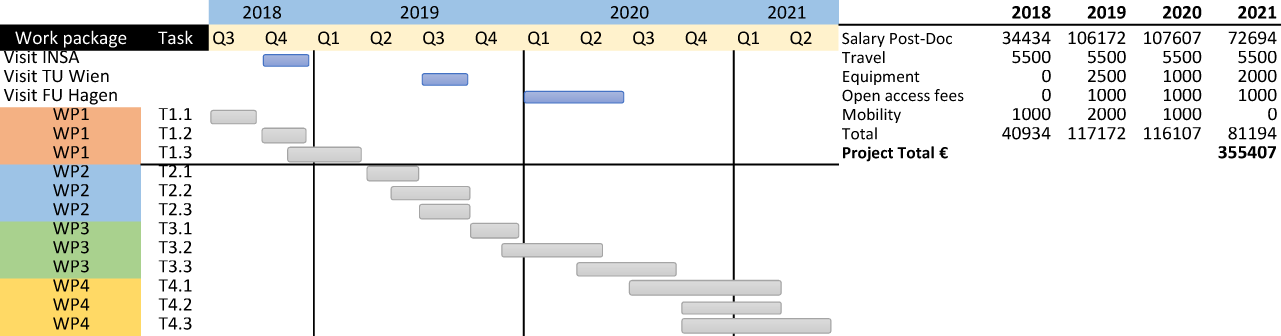
\includegraphics[scale=0.7]{fig/schedule.png}
	\caption{The schedule of the research work is summarized in this figure and the budget of the project in Euros}
	\label{fig:schedule}
\end{figure}
% \paragraph{Budget.}
% The budget of the project is defined in Table 1.\\
% \begin{wraptable}{r}{8cm}
% \vspace{-1.3cm}
% \small
% \begin{tabular}{ | l | c | c |c |c |}
% \hline
% & {\textbf{2018}} & {\textbf{2019}} & {\textbf{2020}} & {\textbf{2021}} \\ \hline
% {Salary Post-doc} 	& 34434 & 106172 & 107607 & 72694 \\ \hline
% {Travel} 			& 5500 	& 5500 	& 5500 	& 5500  \\ \hline
% {Equipment} 		& 0 	& 2500 	& 1000 	& 2000  \\ \hline
% {Open access fees} 	& 0 	& 1000 	& 1000 	& 1000  \\ \hline
% {Mobility} 			& 1000 	& 2000 	& 1000 	& 0  \\ \hline
% {\textbf{Total}} 	& 40934 & 117172	& 116107 	& 81194  \\ \hline
% {\textbf{Project total}} 	&  & 	&  	& 355407  \\ \hline
% \end{tabular}
% \caption*{Table 1: The budget of the project in euros}
% \label{tab:budget}
% \vspace{-1.5cm}
% \end{wraptable}



\subsection{Work packages}
\paragraph{WP1 -- Defining energy-awareness.}
\begin{wraptable}{r}{9cm}
\vspace{-0.5cm}
\small
\begin{tabular}{ | l |}
\hline
{Task 1.1 Defining self-awareness}  \\ \hline
{Task 1.2 Tool support for introducing self-awareness}  \\ \hline
{Task 1.3 library for introducing self-awareness into applications}\\ \hline
\end{tabular}
\vspace{-0.3cm}
\end{wraptable}
WP1 is inline with the first objective: to include self-awareness into applications (T1.1), this is needed for the applications to express resource requirements.
Firstly we determine which meta-data is needed to properly express the intension of the software.
We determine which details to include in the meta-data, and we put focus on the usability of the meta-data expression.
To increase the usability and to enable automatic self-awareness assessment, we will include tool support for including self-awareness (T1.2).
We intend to expand the functionality of the PREESM tool for this purpose, and this is the main focus in Mobility 1.
Finally we build the backend library (T1.3) for the programmer to easily insert/remove/modify self-awareness in applications.
The library is primarily intended for the C language, but portability to e.g. Python pip is considered in this WP.
Deliverables from this WP are scientific publications and the base implementation of the library backend available as opensource on github together with its documentation.
\paragraph{WP2 -- Interoperability.}
\begin{wraptable}{r}{9.7cm}
\vspace{-0.5cm}
\small
\begin{tabular}{ | l |}
\hline
Task 2.1 Application monitoring and implementation of monitor  \\ \hline
Task 2.2 User interoperability   \\ \hline
Task 2.3 Tool Support and demonstration	\\ \hline
\end{tabular}
\vspace{-0.3cm}
\end{wraptable}
WP2 covers the interoperability and monitoring aspect of the project as discussed in the second objective of this project.
In this WP we solve the problem of interoperability between the programmer (WP1), the application and the runtime system (WP3).
To properly handle dynamic applications, a monitoring framework must continuously obtain the performance state of the energy-aware application at runtime.
The performance of the system shall always be sufficient with respect to the resource requirement set by the programmer (WP1).
In order to minimize the influence of the application, the monitoring framework must be extremely lightweight, and its interface to the application must be simple in order to not affect its usability.
The first challenge to tackle is how the application can be monitored without affecting the functionality or the performance of the system.
State-of-the-art monitoring systems such as the MIT heartbeats \cite{Hoffmann:10} will be evaluated as complementary research to the proposed energy-awareness monitor.
A monitoring interface will be developed and its cross-domain applicability will be evaluated on Android, PC and server systems.
Secondly (T2.2) we intend to allow interoperability between user and runtime system in form of a communications channel.
The user shall be able to easily modify the energy-awareness during runtime by callbacks to the backend library.
We will implement and demonstrate this functionality with a real-world application executing on real hardware (T2.3).
Deliverables from this WP are scientific publications and the implementation of the monitor and interoperability framework available as opensource on github together with its documentation.
We also consider complementary implementation to the base backend library from WP1 if deemed necessary.
\paragraph{WP3 -- Smart-adaption.}
\begin{wraptable}{r}{9.4cm}
\vspace{-0.4cm}
\small
\begin{tabular}{ | l |}
\hline
Task 3.1: Modeling energy consumption and tool support\\ \hline
Task 3.2: Runtime optimization for energy efficiency \\ \hline
Task 3.3: Implementation of runtime controller \\ \hline
\end{tabular}
\vspace{-0.3cm}
\end{wraptable}
The tool providing self-awareness from WP1 and the information from the interoperability monitor in WP2 will be directly utilized in WP3 as input for the adaptive control system.
The main task in WP3 is to define the resource allocation to achieve maximal energy efficiency without performance loss.
We firstly (T3.1) create mathematical models of the underlying system upon which optimization methods are deployed.
Tools for automatically generating models are created to enhance portability between hardware devices such as IoT systems, embedded devices and server platforms.
Feasibility and suitability for deployment on real-world platforms is studied, and the scalability of the methods are investigated.
To be able to support a wide range of hardware devices and dynamic software, we must develop robust optimization methods (T3.2).
Initially we intend to study simulation environments such as Philharmonic and Simulink to gain an overview of feasible optimization methods and approaches. 
The main part of WP3 is the implementation of the control system (T3.3) which is partly completed during Mobility 3.
Included in this task is extensive experimental science to test and evaluate all aspects of the final control system.
In focus is the ability to adapt the hardware resources in very diverse software systems, the accuracy of the resource allocation, the performance of the application and the energy consumption.
Deliverables from this WP are scientific publications and the implementation of the runtime controller available as opensource on github together with its documentation.
We also consider complementary implementation to the base backend library from WP1 if deemed necessary.
\paragraph{WP4 -- A framework for energy-aware programming and demonstrator.}
\begin{wraptable}{r}{9.2cm}
\vspace{-0.4cm}
\small
\begin{tabular}{ | l |}
\hline
Task 4.1: Back-end implementation of programming framework\\ \hline
Task 4.2: Front-end development in form of an Eclipse plug-in \\ \hline
Task 4.3: Single use-cases and Demonstrator\\ \hline
\end{tabular}
\vspace{-0.3cm}
\end{wraptable}
The final stage of the research is to bind the previously created methods into a package usable for the programmer.
Construction of the API framework used for energy-aware programming is defined as the first item in WP4.
This includes the back-end library which is callable from the programming environment, and the front-end in form on an Eclipse plug-in.
The parts of the back-end that has been prototyped in WP1 and WP2 are tied together as a fully functioning product.
% A software library, pragma or other interface is the final deliverable and is the link between the application software and the runtime.
The API and the back-end is a result from the support for self-awareness in WP1, the monitor and interoperability interface in WP2 and the runtime system in WP3.
Additional efforts in this WP is put on supporting interdisciplinary domains of platforms, we will demonstrate the feasibility of using energy-aware programming on both mobile devices and large scale servers,
and the resulting energy savings this approach will bring.
We provide small single use-cases of the functionality of the framework and lastly a large scale demonstrator is created running a complete version of the energy-aware software on an off-the-shelf consumer device such as an Android phone or tablet.
Deliverables from this WP are scientific publications and the implementation of the programming framework as opensource on github together with documentation and as an available Eclipse source.
We also plan to attend industrial sessions and hands-on tutorials to demonstrate the final product.

\section{Research Team and Collaborative Partners}
\paragraph{Merits of research team.}
The PI was awarded the honorary degree for his thesis as well as the \textit{Researcher of the Year award} by AAU for best PhD thesis during the year 2016; this provides a solid ground to start the project from.
The PI has published over 25 high ranking articles in the area of energy-aware software during the past five years and additional articles in various workshops, 
and received the \textit{Best Paper Award} at the 2014 DASIP conference.
Our lab and the PI has worked within several international and national research projects such as ESC, RECOMP, ParallaX and INTERSYS with close ties to Finnish industry like Nokia, ABB, Kone, Ericsson etc.

\paragraph{Key national and international collaboration.}
The research in the thesis of the PI consisted of contributions from 17 co-authors in 7 universities in 6 countries.
The cooperation between Prof. Jean-Francois Nezan, INSA de Rennes, and AAU has concentrated on the run-time management of dataflow networks, 
and has been executed through exchange of PhD students.
The previously developed PREESM\footnote{http://preesm.sourceforge.net/website/} tool which was used to determine parallelism in data-flow programs was used in combination with a power optimizer developed by the PI. 
The PI visited INSA de Rennes for 4 months in 2013-2014, and the co-written Best Paper from this visit resulted in the best thesis awards both in AAU for the PI, and in INSA for the co-author.
A cooperation between the PI and Prof. J\"{o}rg Keller at the FernUniversit\"{a}t in Hagen started in 2014, after which the PI was hired as a post-doc researcher for 18 months.
The cooperation with FernUni is currently very active in the field of energy efficient scheduling for multi-core systems. 
One scientific journal and four proceedings and four Master's theses was published during this cooperation.
The PI has been cooperating with the Electronic Commerce Group in TU Wien led by Prof. Ivona Brandi\'{c} since spring 2015 inside the COST action IC1305 framework. 
Work on cost and energy efficient cloud scheduling was done by extending the Philharmonic cloud simulator\footnote{http://philharmonic.github.io/} created at TU Wien with a multi-core model developed by the PI at AAU. 
A journal has been published in the high ranking IEEE Transactions journal as a result of this cooperation.
The PI has an active collaboration with Prof. Alexandra Jimborean from Uppsala University in Sweden, inside the MCC workshop group.
Their lab group is working on compile-time and runtime code analysis and transformation for performance and energy efficiency using LLVM, and they were, together with the PI, a key partner in the 2017 H2020 call on low power programming.
Since UU is geographically near, we plan ad-hoc visit without a defined timeline at this moment.
% Her group has developed a monitoring and feedback system for re-organizing instruction calls based on their memory intensity.
The PI is actively involved in minor collaborations with many universities and companies such as Uni. Carlos III Madrid, Uni. Gronningen, TU Eindhoven, Uni. Turku, NTNU Trondheim, Uni. Tirana, Elisa Inc., Treelogic Inc., Ingenarius Inc., Comsel systems Inc., Hipperos Inc., RISE Inc., TXT E-Solutions Inc.
Additional collaboration and mobilities is expected among these partners.


\section{Research Careers and Research Training}
\label{sec:cooperation}
\paragraph{Advancing the research career of the applicant and researcher training.}
With the advancement of this project, the aim of the PI and the university is to claim the leading role for energy-aware software research in Europe.
The advancement of the career is needed to build stronger networks of leading European partners in the area of energy efficiency in computer systems,
and to create a strong collaboration to maximize the impact and breakthrough to lowering the energy consumption of computer systems world-wide.
The PI stresses the importance of energy efficiency in programming in university teaching, and we will put this niche into practice to attract students from many disciplines and countries.
Combined with the international co-operation, exchange period and close interaction between participating institutes, the project gives the PI good basis to proceed in the academic career after the project with a docentship specialized in energy-aware software as a goal.

\section{Mobility Plan for the Funding Period}
The mobilities among the main partners are planned as follows and illustrated in Figure \ref{fig:schedule}, but the exact details will be defined later in the project based on the availability of the collaborators and their time schedule.

\textit{Mobility 1 }
\includegraphics[width=0.4cm]{fig/fra.png} The PI will visit Prof. Jean-Francois Nezan for 3 months in WP1 to gain knowledge about tool support for introducing energy-awareness in applications.
With a clear definition of self-awareness in T1.1, we expect this mobility to greatly improve T1.2 with the proven expertise of INSA in tool programming.
We intend extend the PREESM tool with the support for energy-awareness.
This mobility is crucial to form the link between the programmer and the software library while still keeping the programmability and complexity to the user low. 
The utilization of PREESM is expected in form of a demonstration environment for WP4.\smallskip

\textit{Mobility 2 }
\includegraphics[width=0.4cm]{fig/aus.png} The PI will visit Prof. Ivona Brandi\'{c} for 3 months in the end of WP2 after the structure of the framework has been established in WP1 in order to adapt and evaluate our framework in cloud environments. 
Special focus will be put on the coordination of resource utilization between computing nodes on a multi-server based infrastructure.
We will evaluate the scalability of the interoperability aspect in the cloud simulator Philharmonic developed at TU Wien, particularly to prove that our methods are sound when scaling up the system to several thousands of servers. 
If needed, we will add support to Philharmonic as part of this mobility.
By studying results from large scale datacenter simulations, we expect to gain valuable knowledge for the implementation of the runtime system in WP3. \smallskip

\textit{Mobility 3 }
\includegraphics[width=0.4cm]{fig/ger.png} The PI will visit Prof. J\"{o}rg Keller for 6 months in the middle of WP3 for support on the energy optimization in WP3 and the construction of the controller in WP3.
The lab group in FernUni has a long and impressive track record in power management systems, 
and their knowledge is needed to link the resource demands stated in WP1 with the actual actuation in form of resource allocation.
Scalability in control algorithms is of special focus to support the full range of computer systems.

\bibliographystyle{alpha}
{\footnotesize
\bibliography{sample}}

%----------------------------------------------------------------------------------------


\end{document}